\documentclass[11pt]{article}
\usepackage[english]{babel}
\usepackage{natbib}
\usepackage{url}
\usepackage[utf8x]{inputenc}
\usepackage{amsmath}
\usepackage{graphicx}
\graphicspath{{images/}}
\usepackage{parskip}
\usepackage{fancyhdr}
\usepackage{vmargin}
\usepackage{caption}
\usepackage{subcaption}

\setmarginsrb{3 cm}{2.5 cm}{3 cm}{2.5 cm}{1 cm}{1.5 cm}{1 cm}{1.5 cm}

\title{Robocon 2018 Project Report}% Title
\author{Abhishek, Nitik, Raunak, Shibalik, Shubham, Sarthak, Rakshit, Vivek, Faizan}% Author
\date{\today}% Date

\makeatletter
\let\thetitle\@title
\let\theauthor\@author
\let\thedate\@date
\makeatother

\pagestyle{fancy}
\fancyhf{}
% \rhead{\theauthor}
\lhead{\thetitle}
\cfoot{\thepage}

\begin{document}

%%%%%%%%%%%%%%%%%%%%%%%%%%%%%%%%%%%%%%%%%%%%%%%%%%%%%%%%%%%%%%%%%%%%%%%%%%%%%%%%%%%%%%%%%

\begin{titlepage}
    \centering
    \vspace*{0.5 cm}
%     \includegraphics[scale = 0.75]{}\\[1.0 cm]   % University Logo
    \textsc{\LARGE Indian Institute of Technology, Kanpur}\\[1 cm]   % University Name
%     \textsc{\Large something}\\[0.5 cm]               % Course Code
    \rule{\linewidth}{0.2 mm} \\[0.4 cm]
    { \huge \bfseries \thetitle}\\
    \rule{\linewidth}{0.2 mm} \\[1 cm]
    	\textsc{Team Members:}\\
    {\large \theauthor}\\[0.5 cm]
    	\textsc{\textbf{Team Lead:} Suraj Mishra}\\
        \textsc{\textbf{Mentor:} Prof. Ashish Dutta}\\[0.5 cm]
    {\large \thedate}\\[2 cm]
 
    \vfill
    
\end{titlepage}

%%%%%%%%%%%%%%%%%%%%%%%%%%%%%%%%%%%%%%%%%%%%%%%%%%%%%%%%%%%%%%%%%%%%%%%%%%%%%%%%%%%%%%%%%

\tableofcontents
\pagebreak

%%%%%%%%%%%%%%%%%%%%%%%%%%%%%%%%%%%%%%%%%%%%%%%%%%%%%%%%%%%%%%%%%%%%%%%%%%%%%%%%%%%%%%%%%

\section{Problem Statement}
The precise aim of our bot is to accurately throw shuttlecocks (design and dimension specified) through rings kept at a certain distance away and high up in the air.

There are two bots: one controlled manually and the other autonomously.
The manual bot has to pick up the shuttlecock from loading zone and give it to the autonomous bot.

The autonomous bot has to throw the shuttlecock through three throwing zones TZ1, TZ2, TZ3 through three hoops one after the other. It can only move to the next throwing zone once it has successfully thrown the shuttlecock in the current throwing zone.

To win the round you have to gain maximum points or achieve rong bay.
To achieve rong bay, you have to clear the first two throwing zones, and then from TZ3, throw the golden shuttlecock through the golden hoop and make it fall on the golden bowl. This achieves ultimate knockout.

\pagebreak

% \section{Overall Strategy}
% Describe it \\

\pagebreak

\section{Mechanical Subsystem}
\subsection{Autonomous Robot}
The chassis designed by the previous team requires many modifications. Our prime focus is on rebuilding the entire basic structure through dynamic CAD modeling and correcting it with supports and external features.
We also attach the entire wheel assembly for the bot, with mecanum wheels. When deciding the wheels we would use for locomotion, we chose mecanum over omni wheels. This is primarily because mecanums are also more efficient in forward and reverse direction while still providing lateral mobility, whereas for omni wheels there is skidding in the bot's lateral movement. Also mecanum wheels will have a firmer grip over the surface.

\begin{figure}[!htb]
\centering
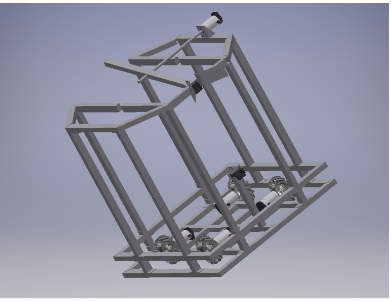
\includegraphics[scale=0.7]{chassis.png}
\end{figure}

\subsection{Throwing Mechanism}
The integration of entire throwing assembly consists primarily of the gripper and motor component. For our throwing mechanism, we had to decide among 2 approaches. For a pneumatics based approach, the existing chassis was incompatible. Also, the chassis was unable to sustain jerks and moved out of plane. Thus this strategy was unsustainable. Thus we decided to use a motor-based strategy, with which the chassis was compatible. For a maxon motor, it can do the throw in 2 rotations.

Now we describe the motor mechanism: 
The main arm is attached to the maxon motor. The entire arm,  attached with the gripper, would be rotated by the motor.
After gaining the necessary angular velocity, the gripper releases the string at a particular angle. This would be determined by the simulation and calculation according to the height and distance of the hoop and throwing gripper.

\begin{figure}[!htb]
\centering
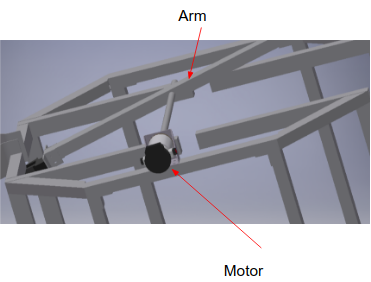
\includegraphics[scale=0.8]{thrower.png}
\end{figure}

\subsection{Manual Robot}
	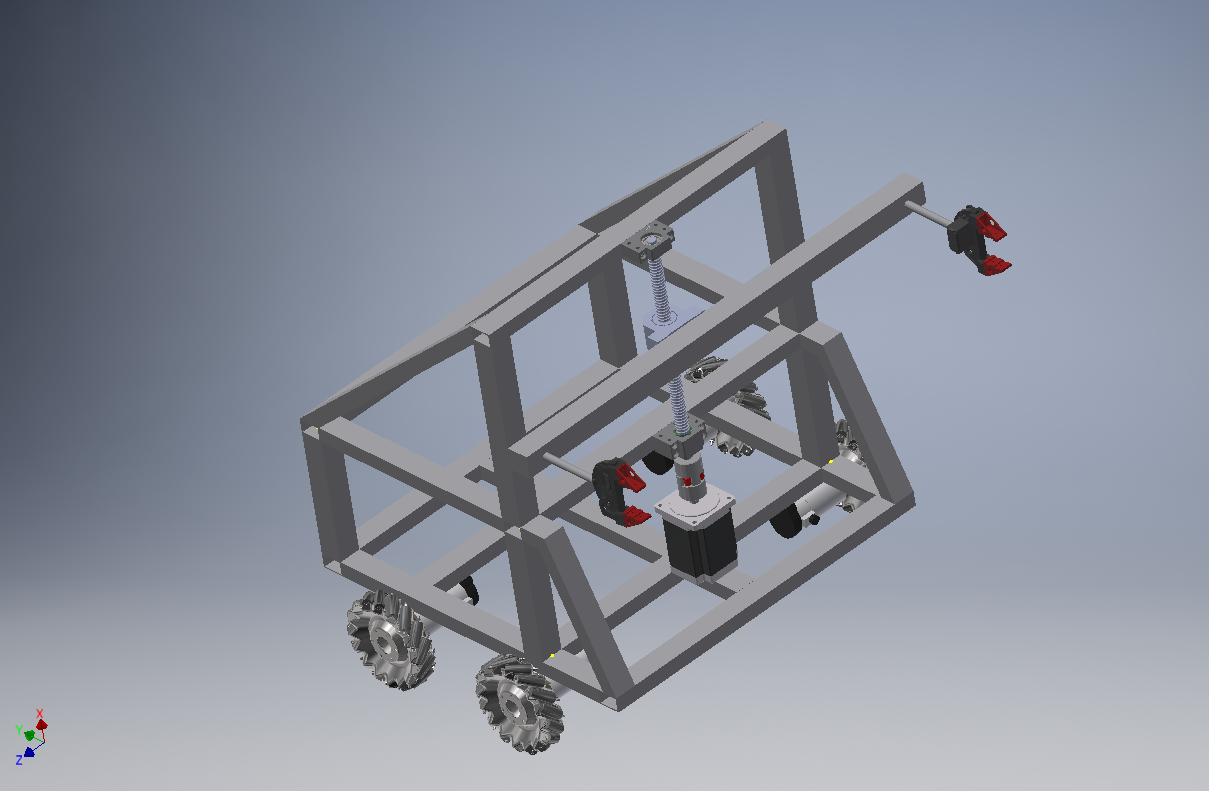
\includegraphics[scale=0.4]{manual.png}
	The Task of this robot is to grab the rack carrying $4$ shuttlecocks. Then the autonomous bot will take shuttlecocks one by one: since the dimension of shuttlecock is $120$mm in diameter so we have to accordingly set the spacing between the grippers.

	 There is a upward motion of the the rack also. We will do this by using a ball screw.
	
	In this bot we are using mecanum wheels because the ball which we are transferring has to be centrally aligned so by using simple wheels we can not do it. So to enable left and right motion we are using mecanum wheels.
    
Our design enables directional supporters to guide the manual robot in placing the shuttlecock. The manual bot holds the shuttlecock through a gripper. After guiding the shuttlecock into the gripper of autonomous bot, its gripper closes to hold the tail of the shuttlecock. A figure depicting this is as follows:

% \begin{figure}[!htb]
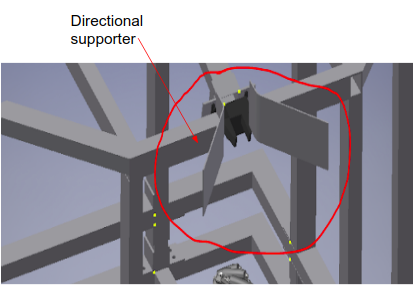
\includegraphics[scale=0.8]{transfer.png}
% \end{figure}

\pagebreak

\section{Electrical Subsystem}
\subsection{Components used}
\subsubsection{RPI}
\begin{itemize}
\item{Quad Core 1.2GHz Broadcom BCM2837 64bit CPU}
\item{1GB RAM}
\item{BCM43438 wireless LAN and Bluetooth Low Energy (BLE) on board}
\item{100 Base Ethernet}
\item{40-pin extended GPIO}
\item{4 USB 2 ports}
\item{4 Pole stereo output and composite video port}
\item{Full size HDMI}
\item{CSI camera port for connecting a Raspberry Pi camera}
\item{DSI display port for connecting a Raspberry Pi touchscreen display}
\item{Micro SD port for loading your operating system and storing data}
\item{Upgraded switched Micro USB power source up to 2.5A}
\end{itemize}
\subsubsection{Microcontrollers(Arduino UNO)}
\begin{itemize}
\item{Operating voltage : 5V}
\item{Recommended input voltage : 7-12 V}
\item{Input voltage limits : 6-20 V}
\item{Analog Input pins : 6 (A0-A5)}
\item{Digital I/O pins : 14 }
\item{DC current on I/O pins : 40 mA}
\item{DC current on 3.3V pin : 50 mA}
\item{Flash memory : 32KB}
\item{SRAM : 2 KB}
\item{EEPROM : 1 KB}
\item{Frequency : 16 MHz}
\end{itemize}
\subsubsection{Motors}
{We need high torque and rotation speed so we are using maxon motors and for low torque we use dc motors}
\begin{itemize}
\item{Maxon Motors}
\item{DC Motors}
\end{itemize}
\subsubsection{Hercules DC Motor Drivers}
\begin{itemize}
\item{Voltage : 6V-24V}
\item{Current : 16 Amp}
\item{Operating pins in arduino : PWM ,IN1 ,IN2}
\item{DG1/DG2 : To detect temperature and short-circuit faults}
\item{CS : Connected through AD0 pin of arduino}

\end{itemize}
\subsection{Printed Circuit Board and Embedded system}
Embedded systems form the crux of the electrical design of any robot . It must be designed with accuracy and in a quite flexible and real time way. 

For this the software ALTIUM was used.
\subsubsection{Advantages of ALTIUM}
\begin{itemize}
\item{Dynamic board designing} 
\item{Libraries available for use provided by competent manufacturers.}
\item{Real time features actually applicable in PCB designing}
\item{Easy Editing possible}
\end{itemize}
Getting started with pcb designing
\subsubsection{Libraries}
 Libraries form an integral part of designer. Libraries are storehouses containing all the components required for embedded systems design.
Components cannot be directly accessed in altium. Also they do not come pre-installed.
Every design has a set of characteristic components linked with it. So, those specific components are located in specific libraries.
Altium has an online documentation for all the libraries required. However, for basic circuit design components libraries Miscellaneous Devices.IntLib and Miscellaneous Connectors. Intlib         
\url {https://techdocs.altium.com/display/ADOH/Download+Libraries}
\subsubsection{Placing components}
It's important to spend a lot of time on component placement to meet mechanical requirements and to group circuits together. The board has a lot of break-out boards tied together so grouping circuits isn't as crucial. The big issue mechanically is fitting everything on the board size that is allowed by Altium. I created packages for all of the components and placed them below. The only issue I had was that two of the ball caster screws interfere with the battery hold plastic, so the battery holder will either be nudged up because it's resting on the screws, or I can skip the two screws and rely on the front two. The line sensor will actually be connected with a series of headers because it has to be very close to the floor. Since I didn't have room underneath the board, it will have to be soldered to the top with a right angle connector and come off the front of the robot.
\subsubsection{Routing key-nets}
We route the important connections manually below, such as power, motor, and motor control. The trace width for power should be as large as possible to limit the voltage drop. If possible, it's best to route all of the traces manually so you know what's happening with the signals. For signals such as low-speed digital connections and other non-critical nets the auto-router can be a great time saver. I did not route the ground because I plan to use a ground plane to connect grounds together. The yellow lines shown below are called "ratsnest" lines and they show which connections have yet to be made. They are useful for manual routing to see where the net should go.
\subsubsection{Clean-up and Ground pour}
It's important to run a DRC check because the auto-router can make mistakes and leave little traces around that shouldn't be there
\subsubsection{Ground Plane}
The ground plane needs to be stitched together using ground vias. This minimizes capacitive coupling between the layers which can cause issues with analog and RF circuitry. More importantly for this robot though is that it reduces the loops and length that the return current needs to take to make it back to the battery. It also allows areas that the plane couldn't reach because of signal traces to be filled.

\pagebreak
\section{Software Subsystem}

All the code described below can be found in multiple branches of the github repository at \url{https://github.com/RoboticsClubIITK/robocon-2018}.

\subsection{Line Following}
This is required to guide the autonomous robot between throwing zones. We identify the midpoint of the line beneath the robot and move based on the error in trajectory. A simple logitech camera should be sufficient for this purpose, and we plan to add an LED to fix lighting issues.

For testing purposes we will use an arduino. Then we have to set an communication between arduino and OpenCV so for this we use inbuilt serial library of python by which we can establish a interactive serial communication between arduino and opencv code.

So firstly we make contours of line and according to these contour showing deviation from midpoint of frame we command the bot to take turns

% 	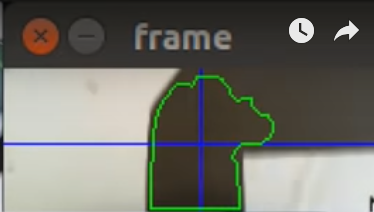
\includegraphics[scale=0.5]{line_follow1.png}
% 	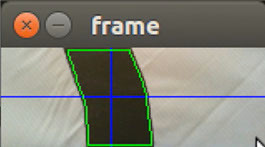
\includegraphics[scale=0.75]{line_follow2.png}
    
\begin{figure}[!htb]
\centering
\begin{subfigure}{.5\textwidth}
  \centering
  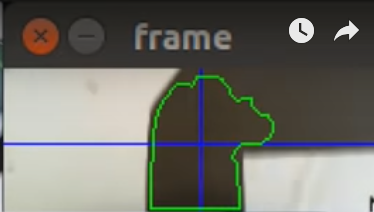
\includegraphics[width=.8\linewidth]{line_follow1.png}
\end{subfigure}%
\begin{subfigure}{.5\textwidth}
  \centering
  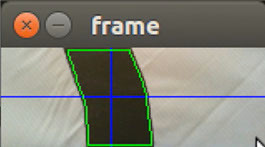
\includegraphics[width=.8\linewidth]{line_follow2.png}
\end{subfigure}
\caption{Midpoint Detection with Line Following}
\label{fig:test}
\end{figure}

In this main task is to reduce the noise and correctly map the virtual pixels into real distances and accordingly calculate angular speeds of both wheels to make certain turns and at what distances before we should  make turn so bot does not lost from its path.

So we tackled noise problem by putting a light which can reduce noise and bot can detect line clearly.

Here we also faced the difficulty in case the line was lost from camera scope. How could we bring the bot back on the line.

\subsection{Image Processing (OpenCV)}
The first step is to get input from the camera. Previously we were planning to use Intel RealSense camera for the same but due to issues with compatibility with other softwares, and lack of sufficient documentation, we plan to use the Kinect as of now.

In the beginning to get acquainted with OpenCV, we worked on contour detection of moving objects. By applying a bilateral filter, followed by Canny, we identified contours using two methods: the findContours function, and approximating the object as a polygon. To understand whether this object is a circle, we set a minimum limit on the number of sides of the polygon, as well as the area of the figure. This also helped eliminate extremely small objects. This method identified general contours, which we expanded upon later:

The ultimate aim here is to understand whether the ball went through the hoop or not. We could track the ball and identify whether it will do so to help us decide whether to move from one throwing zone to another. On the other hand, having such a lack of confidence in our throwing mechanism is bound to cost us the win in an actual competition. Thus it is better to create a foolproof throwing mechanism, as the winning teams have, rather than rely on error correction.

Still, if we insist on determining this, we have several strategies in place:

\begin{itemize}
\item{We wrote ball-tracking code which works to a distance of 4-5 meters. This relies on tracking the shuttlecock based on color thresholding. Since the unpredictable background could interfere with this method, we will have to do depth-based background subtraction using a depth camera like the Kinect. The main challenge with this method is that the ring is extremely far away (~6-7 meters), so traditional cameras may not give reliable results.}

\item{We also attempted to do depth detection using stereo vision with two logitech cameras for understanding the process behind this.}

\item{Another method is to use shuttlecocks of different colors, and supply them to the autonomous bot based on if it successfully throws the shuttlecock. We can use color sensors to decide whether to try in the current TZ or move to the next one. The main problem with this method is the extra time wasted to wait for the shot to be completed.}
\end{itemize}

\subsection{ROS and Integration}
To get acquainted with ROS and get started with integration we tried several experiments and completed many tutorials:
\begin{itemize}
\item{We initially worked on coding nodes for basic publishers and subscribers, and how they work with topics. We also explored the basic server-client architecture in ROS and used it to generate messages and subscribe to them in this area. Finally we moved on to creating a publisher that will publish for the node turtlesim and move the turtle in a desired path hardcoded by us.}
\item{For integrating the image processing portion, we wrote nodes for interfacing with the usb\_cam node, and publishing and subscribing to the feed that is generated. We displayed this using RViz, as well as by publishing the feed to the camera/image\_raw topic. After obtaining the image, we used the image\_transport and cvBridge libraries to link the feed with the OpenCV code written earlier. Then the feed can be processed and later, displayed by publishing to a topic or simply using OpenCV functions for the same.}
\item{We decided to use the arduino for initial testing purposes. In this case, we worked on interfacing with the rosserial node. We coded simple publishers and subscribers for the arduino to understand how messages are passed using this device with ROS. We also wrote code for servo motor control and usage of ultrasonic sensor with the Arduino, which activates or deactivates based on the distance of the object before it. We plan to link the arduino with the motor driver and use it to move the bot as well as the throwing mechanism based on vision and sensory input. 
}
\end{itemize}

\pagebreak

\section{Future Plan}
\subsection{Mechanical}
\begin{itemize}
\item{Set up throwing mechanism}
\item{Test with arduino and hoop setup}
\item{Simultaneously complete hardcoded locomotion}
\end{itemize}

\subsection{Electrical}
\begin{itemize}
\item{Plan to integrate all sensors and components over an integrated board which would be linked to a discreet processing unit}
\item{The PCB would be having all hood connections with directional linkings to reduce replication and cross-linking errors}
\item{Use Altium as the prime designing software for embedded sytstems and PCB Designs}
\item{Test with arduino and hoop setup}
\item{Simultaneously complete hardcoded locomotion}
\end{itemize}
\subsection{Software}
\begin{itemize}
\item{The code for conditional movement and throwing the shuttlecock based on input from vision and sensors}
\item{Hardcoding path and angle for the bot based on dimensions of the arena}
\item{Using TF for integrating throwing and motion of bot}
\item{Simulation with Gazebo}
\item{Integrating NUC/Odroid microprocessor with ROS and vision}
\end{itemize}
\end{document}
